\chapter{矩阵与行列式}

矩阵是线性代数的基本语言，也是模形式理论中矩阵群、线性分式变换与 Hecke 算子的共同背景。本章从最基础的矩阵运算出发，系统讨论初等变换、行列式、逆矩阵以及分块矩阵。虽然这些内容在初等代数中已经出现过，但我们将尽量从定义出发，给出完整证明，并强调今后反复使用的结构性观点：
\begin{itemize}
  \item 矩阵乘法编码了线性变换的复合；
  \item 初等矩阵把“消元法”变成了矩阵乘法；
  \item 行列式刻画了体积伸缩、可逆性与有向面积；
  \item $\SL_2(\Z)$ 中的矩阵正是模形式最核心的对称对象。
\end{itemize}

本章默认矩阵的元素取自一个数域或更一般的交换域 $\F$（典型地可以取 $\Q,\R,\C$）。若无特别说明，所有矩阵都在同一个域 $\F$ 上讨论。

\section{矩阵的基本运算}

\subsection{矩阵与记号}

\begin{definition}
设 $m,n\in\N^+$。一个 \emph{$m\times n$ 矩阵} 是一个按矩形排布的元素族
\[
A=(a_{ij})_{1\le i\le m,\,1\le j\le n},\qquad a_{ij}\in \F.
\]
全体 $m\times n$ 矩阵组成的集合记为 $\Mat_{m,n}(\F)$。当 $m=n$ 时，称之为 \emph{$n$ 阶方阵}，记为 $\Mat_n(\F)$。
\end{definition}

通常我们把矩阵写成
\[
A=\mat{a_{11}&a_{12}&\cdots&a_{1n}\\
         a_{21}&a_{22}&\cdots&a_{2n}\\
         \vdots&\vdots&\ddots&\vdots\\
         a_{m1}&a_{m2}&\cdots&a_{mn}}.
\]
第 $i$ 行第 $j$ 列的元素称为 $A$ 的 $(i,j)$ 元，记为 $a_{ij}$。如果所有非对角元都为 $0$，则称该矩阵为 \emph{对角矩阵}；若对角元全为 $1$，则称其为 \emph{单位矩阵}，记为 $\Id_n$ 或简记为 $I_n$。

\begin{example}
在 $\Mat_{2,3}(\R)$ 中，矩阵
\[
A=\mat{1&0&-2\\3&4&5}
\]
有两行三列。其第一行是 $(1,0,-2)$，第三列是 $\mat{-2\\5}$。
\end{example}

\subsection{加法与数乘}

\begin{definition}
设 $A=(a_{ij}),B=(b_{ij})\in\Mat_{m,n}(\F)$，$\lambda\in\F$。定义
\[
A+B=(a_{ij}+b_{ij}),\qquad \lambda A=(\lambda a_{ij}).
\]
分别称为 \emph{矩阵加法} 与 \emph{数乘}。
\end{definition}

这些运算都是逐项进行的，因此和向量的加法、数乘完全类似。

\begin{proposition}
集合 $\Mat_{m,n}(\F)$ 在矩阵加法与数乘下构成一个 $\F$-向量空间。具体地，对任意 $A,B,C\in\Mat_{m,n}(\F)$ 与 $\lambda,\mu\in\F$，有
\begin{align*}
A+B&=B+A,\\
(A+B)+C&=A+(B+C),\\
A+0&=A,\\
A+(-A)&=0,\\
\lambda(A+B)&=\lambda A+\lambda B,\\
(\lambda+\mu)A&=\lambda A+\mu A,\\
(\lambda\mu)A&=\lambda(\mu A),\\
1\cdot A&=A.
\end{align*}
\end{proposition}

\begin{proof}
每一条都可逐项验证。例如，若 $A=(a_{ij}),B=(b_{ij}),C=(c_{ij})$，则
\[
((A+B)+C)_{ij}=(a_{ij}+b_{ij})+c_{ij}=a_{ij}+(b_{ij}+c_{ij})=(A+(B+C))_{ij},
\]
故 $(A+B)+C=A+(B+C)$。其余性质都来自域 $\F$ 中加法与乘法的相应性质，完全类似。
\end{proof}

\begin{example}
设
\[
A=\mat{1&2\\3&4},\qquad B=\mat{-1&0\\5&2}.
\]
则
\[
A+B=\mat{0&2\\8&6},
\qquad 3A=\mat{3&6\\9&12}.
\]
\end{example}

\subsection{矩阵乘法}

矩阵乘法比加法更重要，也更微妙。它不是逐项相乘，而是“行与列配对求和”。

\begin{definition}
设 $A=(a_{ij})\in\Mat_{m,n}(\F)$，$B=(b_{jk})\in\Mat_{n,r}(\F)$。定义它们的乘积 $AB\in\Mat_{m,r}(\F)$ 为
\[
(AB)_{ik}=\sum_{j=1}^n a_{ij}b_{jk}.
\]
也就是说，第 $i$ 行第 $k$ 列元素由 $A$ 的第 $i$ 行与 $B$ 的第 $k$ 列按对应项相乘再求和得到。
\end{definition}

矩阵乘法的定义要求前一个矩阵的列数等于后一个矩阵的行数。这一相容条件非常重要。

\begin{example}[行乘列]
设
\[
A=\mat{1&2&-1\\0&3&4},\qquad B=\mat{2&1\\-1&0\\5&2}.
\]
则 $A\in\Mat_{2,3}(\F)$，$B\in\Mat_{3,2}(\F)$，故 $AB\in\Mat_{2,2}(\F)$。计算得
\[
AB=\mat{
1\cdot2+2\cdot(-1)+(-1)\cdot5 & 1\cdot1+2\cdot0+(-1)\cdot2\\
0\cdot2+3\cdot(-1)+4\cdot5 & 0\cdot1+3\cdot0+4\cdot2
}
=\mat{-5&-1\\17&8}.
\]
\end{example}

从结构上看，$AB$ 的第 $(i,k)$ 元就是 $A$ 的第 $i$ 行与 $B$ 的第 $k$ 列的点积。这个“行乘列”的思想会在后文不断出现，尤其是在解释线性变换复合与分块矩阵乘法时。

\begin{proposition}[矩阵乘法的基本性质]
设相应的矩阵乘积都有意义，则有：
\begin{enumerate}[label=(\arabic*)]
  \item 结合律：$(AB)C=A(BC)$；
  \item 左分配律：$A(B+C)=AB+AC$；
  \item 右分配律：$(A+B)C=AC+BC$；
  \item 与数乘相容：$(\lambda A)B=\lambda(AB)=A(\lambda B)$；
  \item 单位矩阵满足 $I_mA=A=AI_n$（其中 $A\in\Mat_{m,n}(\F)$）。
\end{enumerate}
\end{proposition}

\begin{proof}
只证明最关键的结合律，其余各条都可由定义直接验证。

设 $A\in\Mat_{m,n}(\F)$，$B\in\Mat_{n,r}(\F)$，$C\in\Mat_{r,s}(\F)$。对任意 $1\le i\le m$，$1\le k\le s$，有
\begin{align*}
((AB)C)_{ik}
&=\sum_{\ell=1}^r (AB)_{i\ell}c_{\ell k}
 =\sum_{\ell=1}^r\Bigl(\sum_{j=1}^n a_{ij}b_{j\ell}\Bigr)c_{\ell k}\\
&=\sum_{j=1}^n\sum_{\ell=1}^r a_{ij}b_{j\ell}c_{\ell k}
 =\sum_{j=1}^n a_{ij}\Bigl(\sum_{\ell=1}^r b_{j\ell}c_{\ell k}\Bigr)\\
&=\sum_{j=1}^n a_{ij}(BC)_{jk}
 =(A(BC))_{ik}.
\end{align*}
故 $(AB)C=A(BC)$。

再看左分配律：
\[
(A(B+C))_{ik}=\sum_{j=1}^n a_{ij}(b_{jk}+c_{jk})=\sum_{j=1}^n a_{ij}b_{jk}+\sum_{j=1}^n a_{ij}c_{jk}=(AB+AC)_{ik}.
\]
右分配律与数乘相容的证明同理。

最后，$(I_mA)_{ij}=\sum_{k=1}^m (I_m)_{ik}a_{kj}=a_{ij}$，因为只有 $k=i$ 时 $(I_m)_{ik}=1$，其余为 $0$。同理 $AI_n=A$。
\end{proof}

\begin{remark}
和普通数乘不同，矩阵乘法一般 \emph{不交换}。即使 $AB$ 与 $BA$ 都有意义，通常也有 $AB\ne BA$。
\end{remark}

\begin{example}[矩阵乘法不交换]
取
\[
A=\mat{1&1\\0&1},\qquad B=\mat{1&0\\1&1}.
\]
则
\[
AB=\mat{2&1\\1&1},\qquad BA=\mat{1&1\\1&2}.
\]
因此 $AB\ne BA$。

更极端地，可能出现 $AB=0$ 但 $BA\ne 0$。例如
\[
A=\mat{1&-1\\1&-1},\qquad B=\mat{1&1\\1&1}.
\]
则
\[
AB=\mat{0&0\\0&0},\qquad BA=\mat{2&-2\\2&-2}.
\]
这表明“消去律”对矩阵乘法并不自动成立。
\end{example}

\subsection{转置}

\begin{definition}
设 $A=(a_{ij})\in\Mat_{m,n}(\F)$。把 $A$ 的行与列交换得到的 $n\times m$ 矩阵称为 $A$ 的 \emph{转置}，记为 $A^T$，即
\[
(A^T)_{ij}=a_{ji}.
\]
\end{definition}

\begin{example}
若
\[
A=\mat{1&2&3\\4&5&6},
\]
则
\[
A^T=\mat{1&4\\2&5\\3&6}.
\]
\end{example}

\begin{proposition}[转置的性质]
设各矩阵大小相容，则有：
\begin{enumerate}[label=(\arabic*)]
  \item $(A^T)^T=A$；
  \item $(A+B)^T=A^T+B^T$；
  \item $(\lambda A)^T=\lambda A^T$；
  \item $(AB)^T=B^TA^T$。
\end{enumerate}
\end{proposition}

\begin{proof}
前三条直接由定义验证。例如
\[
((A^T)^T)_{ij}=(A^T)_{ji}=a_{ij}.
\]

对第四条，设 $A\in\Mat_{m,n}(\F)$，$B\in\Mat_{n,r}(\F)$。则
\begin{align*}
((AB)^T)_{ki}&=(AB)_{ik}=\sum_{j=1}^n a_{ij}b_{jk},\\
(B^TA^T)_{ki}&=\sum_{j=1}^n (B^T)_{kj}(A^T)_{ji}=\sum_{j=1}^n b_{jk}a_{ij}.
\end{align*}
因为域中乘法交换，所以这两个和相等，故 $(AB)^T=B^TA^T$。
\end{proof}

\begin{definition}
若方阵 $A$ 满足 $A^T=A$，则称 $A$ 为 \emph{对称矩阵}；若满足 $A^T=-A$，则称 $A$ 为 \emph{斜对称矩阵}。
\end{definition}

\begin{example}
矩阵
\[
\mat{2&3\\3&1}
\]
是对称矩阵，而
\[
\mat{0&5\\-5&0}
\]
是斜对称矩阵。
\end{example}

\section{初等变换与初等矩阵}

矩阵计算中最常用的方法之一是 \emph{消元}。它的本质是对矩阵的行或列做一系列简单变换，并保持所关心的结构（例如解集、秩或行列式）有可控变化。

\subsection{三类初等行变换与列变换}

\begin{definition}
设 $A\in\Mat_{m,n}(\F)$。以下三类操作称为 \emph{初等行变换}：
\begin{enumerate}[label=(\arabic*)]
  \item 交换两行；
  \item 用非零数 $\lambda\in\F^\times$ 乘某一行；
  \item 把某一行的 $\lambda$ 倍加到另一行上。
\end{enumerate}
类似地，对列进行完全相同的三类操作，称为 \emph{初等列变换}。
\end{definition}

\begin{example}
设
\[
A=\mat{1&2&3\\4&5&6\\7&8&9}.
\]
对它做初等行变换 $R_3\leftarrow R_3-2R_1$，得到
\[
\mat{1&2&3\\4&5&6\\5&4&3}.
\]
再交换前两行，可得
\[
\mat{4&5&6\\1&2&3\\5&4&3}.
\]
\end{example}

把“以一行的倍数加到另一行”写成符号形式，例如
\[
\mat{1&2&3\\4&5&6\\7&8&9}
\xrightarrow{\ R_3\leftarrow R_3-2R_1\ }
\mat{1&2&3\\4&5&6\\5&4&3},
\]
这正是高斯消元中最常见的一步。

\begin{remark}
解线性方程组时，对增广矩阵做初等行变换并不会改变方程组的解集；这是高斯消元法的基础。关于线性方程组与线性映射的系统讨论将在后续章节展开。
\end{remark}

\subsection{初等矩阵}

\begin{definition}
由单位矩阵 $I_n$ 经过一次初等行变换得到的 $n$ 阶矩阵，称为 \emph{初等矩阵}。
\end{definition}

典型地：
\begin{itemize}
  \item 交换第 $i,j$ 行得到的初等矩阵把 $I_n$ 的第 $i,j$ 行对调；
  \item 把第 $i$ 行乘以 $\lambda\ne 0$ 得到的初等矩阵在第 $i$ 个对角元处是 $\lambda$，其余与 $I_n$ 相同；
  \item 把第 $j$ 行的 $\lambda$ 倍加到第 $i$ 行得到的初等矩阵是在 $I_n$ 的 $(i,j)$ 位置添上 $\lambda$。
\end{itemize}

\begin{example}
在 $3\times 3$ 情形中，
\[
E_1=\mat{0&1&0\\1&0&0\\0&0&1},\qquad
E_2=\mat{1&0&0\\0&5&0\\0&0&1},\qquad
E_3=\mat{1&0&0\\-2&1&0\\0&0&1}
\]
分别对应于：交换第 $1,2$ 行；第 $2$ 行乘以 $5$；把第 $1$ 行的 $-2$ 倍加到第 $2$ 行。
\end{example}

\begin{proposition}[左乘初等矩阵对应行变换]
设 $E\in\Mat_n(\F)$ 是由 $I_n$ 经过一次初等行变换得到的初等矩阵，$A\in\Mat_{n,m}(\F)$。则 $EA$ 正是对 $A$ 做同样的那一次初等行变换所得的矩阵。
\end{proposition}

\begin{proof}
分三类讨论。

\textbf{第一类：交换第 $i,j$ 行。} 设 $E$ 由 $I_n$ 交换第 $i,j$ 行得到。由于 $EA$ 的第 $r$ 行等于 $E$ 的第 $r$ 行与 $A$ 各行的线性组合，而 $E$ 的第 $r$ 行恰是某个标准基行向量，因此 $EA$ 的第 $r$ 行等于 $A$ 的第 $r$ 行（当 $r\ne i,j$）或交换后的对应行（当 $r=i,j$）。故 $EA$ 正是交换了 $A$ 的第 $i,j$ 行。

\textbf{第二类：第 $i$ 行乘以 $\lambda\ne 0$。} 此时 $E$ 与 $I_n$ 只在 $(i,i)$ 处不同，且 $e_{ii}=\lambda$。于是 $EA$ 的第 $i$ 行变成原第 $i$ 行的 $\lambda$ 倍，其余行不变。

\textbf{第三类：把第 $j$ 行的 $\lambda$ 倍加到第 $i$ 行。} 此时 $E=I_n+\lambda E_{ij}$（这里 $E_{ij}$ 表示在 $(i,j)$ 处为 $1$、其余处为 $0$ 的矩阵）。于是 $EA=A+\lambda E_{ij}A$。矩阵 $E_{ij}A$ 的第 $i$ 行等于 $A$ 的第 $j$ 行，其余行全为零，所以 $EA$ 恰好把第 $j$ 行的 $\lambda$ 倍加到了第 $i$ 行。

三种情形皆证。
\end{proof}

\begin{remark}
类似地，若 $E$ 是由 $I_n$ 通过一次初等列变换得到的初等矩阵，而 $A\in\Mat_{m,n}(\F)$，则 $AE$ 等于对 $A$ 做同样的列变换。也就是说，\emph{左乘对应行变换，右乘对应列变换}。
\end{remark}

\begin{proposition}[初等矩阵可逆]
每个初等矩阵都是可逆矩阵，而且其逆矩阵仍是同类型的初等矩阵。
\end{proposition}

\begin{proof}
分别讨论三类情形：
\begin{enumerate}[label=(\arabic*)]
  \item 若 $E$ 对应交换两行，则再交换同样两行一次就回到原矩阵，所以 $E^{-1}=E$。
  \item 若 $E$ 对应把某一行乘以 $\lambda\ne 0$，则其逆操作是把该行乘以 $\lambda^{-1}$，故 $E^{-1}$ 仍是第二类初等矩阵。
  \item 若 $E$ 对应把第 $j$ 行的 $\mu$ 倍加到第 $i$ 行，则逆操作是把第 $j$ 行的 $-\mu$ 倍加到第 $i$ 行，故 $E^{-1}$ 仍是第三类初等矩阵。
\end{enumerate}
因此每个初等矩阵都可逆。
\end{proof}

\begin{proposition}
一个方阵 $A$ 可以通过有限次初等行变换化为单位矩阵，当且仅当 $A$ 可以写成有限个初等矩阵的乘积。
\end{proposition}

\begin{proof}
若 $A$ 经过初等行变换 $E_1,E_2,\dots,E_r$ 化为单位矩阵，则
\[
E_r\cdots E_2E_1A=I_n.
\]
两边左乘逆矩阵，可得
\[
A=E_1^{-1}E_2^{-1}\cdots E_r^{-1}.
\]
由于每个 $E_i^{-1}$ 仍是初等矩阵，所以 $A$ 是初等矩阵的乘积。

反过来，若 $A=E_1E_2\cdots E_r$，则对 $A$ 依次施加与 $E_r^{-1},\dots,E_1^{-1}$ 相应的初等行变换，就可把 $A$ 化为 $I_n$。
\end{proof}

\begin{remark}
有限次初等行变换可以把任意矩阵化为行阶梯形。行阶梯形中非零行的个数称为矩阵的 \emph{秩}，记为 $\rank(A)$。关于秩的系统理论将在下一章讨论，但读者从现在起已经可以把“高斯消元”理解为矩阵结构分析的基本工具。
\end{remark}

\section{行列式的定义与性质}

行列式只对方阵定义。它是一个把矩阵送到标量的函数，用来测量矩阵是否退化，并编码许多深刻的代数与几何信息。

\subsection{排列与 Leibniz 公式}

\begin{definition}
$n$ 个元素的全排列所成的集合记为 $S_n$。对 $\sigma\in S_n$，其符号（或奇偶性）记为 $\sgn(\sigma)\in\{1,-1\}$：若 $\sigma$ 可写成偶数个换位的乘积，则 $\sgn(\sigma)=1$；若只能写成奇数个换位的乘积，则 $\sgn(\sigma)=-1$。
\end{definition}

\begin{definition}[行列式]
设 $A=(a_{ij})\in\Mat_n(\F)$。定义 $A$ 的 \emph{行列式} 为
\[
\det(A)=\sum_{\sigma\in S_n}\sgn(\sigma)\,a_{1\sigma(1)}a_{2\sigma(2)}\cdots a_{n\sigma(n)}.
\]
这一定义也称为 \emph{Leibniz 公式}。
\end{definition}

\begin{remark}
Leibniz 公式中，每一项都从矩阵的每一行、每一列各选出一个元素相乘，然后按排列的奇偶性加上正负号。$n$ 阶行列式一共有 $n!$ 项，因此直接用定义计算只适合小规模矩阵。真正的计算通常依赖于后面要证明的性质。
\end{remark}

\begin{example}[$2\times 2$ 行列式]
当
\[
A=\mat{a&b\\c&d}
\]
时，$S_2$ 中只有恒等排列和换位 $(12)$，故
\[
\det(A)=ad-bc.
\]
这是最熟悉的二阶行列式公式。
\end{example}

\begin{example}[$3\times 3$ 行列式]
设
\[
A=\mat{a&b&c\\d&e&f\\g&h&i}.
\]
则
\begin{align*}
\det(A)
&=aei+bfg+cdh-ceg-bdi-afh.
\end{align*}
这就是三阶行列式的标准展开式。
\end{example}

\subsection{行列式的特征性质}

把矩阵按列写成 $A=(v_1,\dots,v_n)$，其中每个 $v_j\in\F^n$ 是第 $j$ 列。行列式的核心性质是：它对每一列都是线性的，而且当两列相等时为零。

\begin{proposition}[多重线性]
固定除第 $j$ 列外的所有列。则行列式关于第 $j$ 列是线性的。也就是说，对任意 $u,w\in\F^n$ 与 $\lambda,\mu\in\F$，有
\[
\det(v_1,\dots,\lambda u+\mu w,\dots,v_n)
=\lambda\det(v_1,\dots,u,\dots,v_n)+\mu\det(v_1,\dots,w,\dots,v_n).
\]
\end{proposition}

\begin{proof}
在 Leibniz 公式中，每一项都只含第 $j$ 列的一个元素，而且是一次幂。故若把第 $j$ 列写成 $\lambda u+\mu w$，则每一项都可按分配律拆成两部分，整体相加便得到右边的两项之和。这正是关于第 $j$ 列的线性性。
\end{proof}

\begin{proposition}[交错性]
设 $A=(v_1,\dots,v_n)$。
\begin{enumerate}[label=(\arabic*)]
  \item 若 $A$ 有两列相同，则 $\det(A)=0$；
  \item 交换两列，行列式变号；
  \item 若某一列是其余列的线性组合中的重复情况，特别地若某一列为零列，则行列式为零。
\end{enumerate}
\end{proposition}

\begin{proof}
先证 (2)。设 $A'$ 由 $A$ 交换第 $p,q$ 列得到。对 Leibniz 公式中的每个排列 $\sigma$，把它与换位 $(pq)$ 复合，可建立一一对应。由于
\[
\sgn((pq)\sigma)=-\sgn(\sigma),
\]
且交换第 $p,q$ 列正好把每一项中的两个因子互换，所以所有项整体多出一个负号，从而 $\det(A')=-\det(A)$。

由 (2) 立刻得 (1)：若第 $p,q$ 列相同，交换这两列后矩阵不变，但行列式应变号，所以
\[
\det(A)=-\det(A),
\]
故 $2\det(A)=0$。在通常讨论的数域 $\Q,\R,\C$ 上，因 $2\ne0$，遂有 $\det(A)=0$。

对 (3)，若某一列为零列，则由多重线性可立即得行列式为零。更一般地，若某一列与另一列相同，则由 (1) 为零；若某一列是若干列的线性组合，可用多重线性展开，并在含有重复列的项上应用 (1)。
\end{proof}

\begin{proposition}[标准化]
\[
\det(I_n)=1.
\]
\end{proposition}

\begin{proof}
在 Leibniz 公式中，单位矩阵除了主对角线元素外全为零，因此只有恒等排列对应的一项不为零，其值为 $1$。故 $\det(I_n)=1$。
\end{proof}

下面给出一个极为重要的唯一性定理。它说明：\emph{行列式是唯一的标准化交错多线性函数。}

\begin{theorem}[行列式的刻画]
设 $\Phi:(\F^n)^n\to\F$ 是关于 $n$ 个向量的函数，满足：
\begin{enumerate}[label=(\arabic*)]
  \item 对每个变量都线性；
  \item 若有两个变量相等，则 $\Phi=0$；
  \item $\Phi(e_1,\dots,e_n)=1$，其中 $e_1,\dots,e_n$ 是标准基。
\end{enumerate}
则对任意列向量 $v_1,\dots,v_n\in\F^n$，都有
\[
\Phi(v_1,\dots,v_n)=\det(v_1,\dots,v_n).
\]
更一般地，若不要求 (3)，则
\[
\Phi(v_1,\dots,v_n)=\Phi(e_1,\dots,e_n)\det(v_1,\dots,v_n).
\]
\end{theorem}

\begin{proof}
把每个向量按标准基展开：
\[
v_j=\sum_{i=1}^n a_{ij}e_i\qquad (1\le j\le n).
\]
由多重线性，
\[
\Phi(v_1,\dots,v_n)=\sum_{i_1,\dots,i_n}a_{i_11}a_{i_22}\cdots a_{i_nn}\,\Phi(e_{i_1},\dots,e_{i_n}).
\]
若某两个指标相同，则对应的两个基向量相同，由交错性该项为零。因此只有 $(i_1,\dots,i_n)$ 恰好是 $1,\dots,n$ 的一个排列时才可能非零。于是
\[
\Phi(v_1,\dots,v_n)=\sum_{\sigma\in S_n}a_{\sigma(1)1}a_{\sigma(2)2}\cdots a_{\sigma(n)n}\,\Phi(e_{\sigma(1)},\dots,e_{\sigma(n)}).
\]
而由“交换两个变量变号”的事实（它由线性与交错性直接推出），可知
\[
\Phi(e_{\sigma(1)},\dots,e_{\sigma(n)})=\sgn(\sigma)\Phi(e_1,\dots,e_n).
\]
故
\[
\Phi(v_1,\dots,v_n)=\Phi(e_1,\dots,e_n)\sum_{\sigma\in S_n}\sgn(\sigma)a_{\sigma(1)1}\cdots a_{\sigma(n)n}.
\]
由于标量乘法交换，右端正是
\[
\Phi(e_1,\dots,e_n)\det(a_{ij})=
\Phi(e_1,\dots,e_n)\det(v_1,\dots,v_n).
\]
若再用条件 $\Phi(e_1,\dots,e_n)=1$，便得到第一结论。
\end{proof}

\subsection{余子式展开}

\begin{definition}
设 $A=(a_{ij})\in\Mat_n(\F)$。删去第 $i$ 行与第 $j$ 列后得到的 $(n-1)\times(n-1)$ 矩阵记为 $A_{ij}$，其行列式
\[
M_{ij}=\det(A_{ij})
\]
称为 $(i,j)$ \emph{余子式}。再定义
\[
C_{ij}=(-1)^{i+j}M_{ij},
\]
称为 $(i,j)$ \emph{代数余子式}。
\end{definition}

\begin{theorem}[按行按列展开]
设 $A=(a_{ij})\in\Mat_n(\F)$。则对任意固定的 $i$，有
\[
\det(A)=\sum_{j=1}^n a_{ij}C_{ij}.
\]
对任意固定的 $j$，也有
\[
\det(A)=\sum_{i=1}^n a_{ij}C_{ij}.
\]
这分别称为沿第 $i$ 行、沿第 $j$ 列的余子式展开。
\end{theorem}

\begin{proof}
只证按第 $i$ 行展开，按列展开完全类似。

在 Leibniz 公式
\[
\det(A)=\sum_{\sigma\in S_n}\sgn(\sigma)\prod_{k=1}^n a_{k\sigma(k)}
\]
中，按 $\sigma(i)=j$ 分类求和：
\[
\det(A)=\sum_{j=1}^n\sum_{\sigma(i)=j}\sgn(\sigma)\,a_{1\sigma(1)}\cdots a_{i-1,\sigma(i-1)}a_{ij}a_{i+1,\sigma(i+1)}\cdots a_{n\sigma(n)}.
\]
对固定的 $j$，内层和里都含公共因子 $a_{ij}$，提出后，剩下的求和正好是在删去第 $i$ 行和第 $j$ 列后，对 $(n-1)$ 阶矩阵做 Leibniz 求和，只是排列的符号要补上把第 $j$ 列移到第 $i$ 个位置所带来的因子 $(-1)^{i+j}$。因此
\[
\sum_{\sigma(i)=j}\sgn(\sigma)\prod_{k\ne i}a_{k\sigma(k)}=(-1)^{i+j}M_{ij}=C_{ij}.
\]
于是
\[
\det(A)=\sum_{j=1}^n a_{ij}C_{ij}.
\]
证毕。
\end{proof}

\begin{example}
计算
\[
A=\mat{1&2&3\\0&4&5\\1&0&6}
\]
的行列式。沿第一行展开：
\begin{align*}
\det(A)
&=1\cdot\dmat{4&5\\0&6}-2\cdot\dmat{0&5\\1&6}+3\cdot\dmat{0&4\\1&0}\\
&=1\cdot 24-2\cdot(-5)+3\cdot(-4)=22.
\end{align*}
\end{example}

\subsection{行列式的运算性质}

\begin{proposition}[对初等行变换的反应]
设 $A\in\Mat_n(\F)$。
\begin{enumerate}[label=(\arabic*)]
  \item 交换两行，行列式变号；
  \item 某一行乘以 $\lambda$，行列式也乘以 $\lambda$；
  \item 把一行的 $\lambda$ 倍加到另一行，行列式不变。
\end{enumerate}
列变换也有完全类似的结论。
\end{proposition}

\begin{proof}
把矩阵按行看待，行列式同样是关于各行的交错多线性函数（因为 $\det(A)=\det(A^T)$，稍后会证明；或者直接对 Leibniz 公式做相同分析）。因此：
\begin{enumerate}[label=(\arabic*)]
  \item 交换两行会使交错函数变号；
  \item 某一行乘以 $\lambda$，由线性性知整体乘以 $\lambda$；
  \item 若把第 $j$ 行的 $\lambda$ 倍加到第 $i$ 行，则由线性性，新的行列式等于原行列式加上一个“第 $i,j$ 行相同”的行列式，而后者为零，所以值不变。
\end{enumerate}
证毕。
\end{proof}

\begin{proposition}[三角矩阵的行列式]
若 $A=(a_{ij})\in\Mat_n(\F)$ 是上三角矩阵或下三角矩阵，则
\[
\det(A)=a_{11}a_{22}\cdots a_{nn}.
\]
\end{proposition}

\begin{proof}
以 $A$ 为上三角矩阵为例。若某排列 $\sigma\ne \Id$，则存在某个 $i$ 使得 $\sigma(i)<i$。于是 $a_{i\sigma(i)}=0$，因为上三角矩阵在主对角线下方元素全为零。因此 Leibniz 公式中除恒等排列外，其余项全部为零，只剩
\[
\det(A)=a_{11}a_{22}\cdots a_{nn}.
\]
下三角情形同理。
\end{proof}

\begin{theorem}[转置不改变行列式]
对任意 $A\in\Mat_n(\F)$，有
\[
\det(A^T)=\det(A).
\]
\end{theorem}

\begin{proof}
设 $A=(a_{ij})$。由定义
\[
\det(A^T)=\sum_{\sigma\in S_n}\sgn(\sigma)\,a_{\sigma(1)1}a_{\sigma(2)2}\cdots a_{\sigma(n)n}.
\]
令 $\tau=\sigma^{-1}$。由于 $\sgn(\tau)=\sgn(\sigma)$，并且当 $\sigma$ 遍历 $S_n$ 时，$\tau$ 也遍历 $S_n$，故
\[
\det(A^T)=\sum_{\tau\in S_n}\sgn(\tau)\,a_{1\tau(1)}a_{2\tau(2)}\cdots a_{n\tau(n)}=\det(A).
\]
\end{proof}

\begin{theorem}[乘积的行列式]
对任意 $A,B\in\Mat_n(\F)$，有
\[
\det(AB)=\det(A)\det(B).
\]
\end{theorem}

\begin{proof}
固定 $A$，定义函数
\[
\Phi(v_1,\dots,v_n)=\det(Av_1,\dots,Av_n),
\]
其中 $v_1,\dots,v_n\in\F^n$ 视为列向量。由于矩阵乘法对每一列线性，且行列式本身对每一列线性，故 $\Phi$ 对每个变量都是线性的。若 $v_i=v_j$，则 $Av_i=Av_j$，于是 $\Phi(v_1,\dots,v_n)=0$。因此 $\Phi$ 是一个交错多线性函数。

由前面的刻画定理，存在常数 $c$ 使得
\[
\Phi(v_1,\dots,v_n)=c\det(v_1,\dots,v_n).
\]
取 $v_j=e_j$，则
\[
c=\Phi(e_1,\dots,e_n)=\det(Ae_1,\dots,Ae_n)=\det(A).
\]
于是对任意 $B=(v_1,\dots,v_n)$，有
\[
\det(AB)=\Phi(v_1,\dots,v_n)=\det(A)\det(B).
\]
证毕。
\end{proof}

\begin{corollary}
若 $E$ 是初等矩阵，则 $\det(E)$ 分别为：
\begin{enumerate}[label=(\arabic*)]
  \item 第一类初等矩阵：$-1$；
  \item 第二类初等矩阵（某一行乘以 $\lambda$）：$\lambda$；
  \item 第三类初等矩阵：$1$。
\end{enumerate}
\end{corollary}

\begin{proof}
这些结论直接由单位矩阵的行列式和初等行变换对行列式的影响得到。
\end{proof}

\section{逆矩阵与 Cramer 法则}

\subsection{可逆矩阵}

\begin{definition}
设 $A\in\Mat_n(\F)$。若存在 $B\in\Mat_n(\F)$ 使得
\[
AB=BA=I_n,
\]
则称 $A$ 是 \emph{可逆矩阵}，$B$ 称为 $A$ 的 \emph{逆矩阵}，记为 $A^{-1}$。
\end{definition}

\begin{proposition}[逆矩阵的唯一性]
若 $A$ 可逆，则其逆矩阵唯一。
\end{proposition}

\begin{proof}
若 $B,C$ 都是 $A$ 的逆矩阵，则
\[
B=BI_n=B(AC)=(BA)C=I_nC=C.
\]
故逆矩阵唯一。
\end{proof}

\begin{theorem}[可逆判别准则]
对 $A\in\Mat_n(\F)$，以下条件等价：
\begin{enumerate}[label=(\arabic*)]
  \item $A$ 可逆；
  \item $\det(A)\ne 0$。
\end{enumerate}
\end{theorem}

\begin{proof}
先证 (1)$\Rightarrow$(2)。若 $A$ 可逆，则存在 $A^{-1}$ 使得 $AA^{-1}=I_n$。取行列式，利用乘法公式得
\[
\det(A)\det(A^{-1})=\det(I_n)=1.
\]
因此 $\det(A)\ne 0$。

再证 (2)$\Rightarrow$(1)。这需要伴随矩阵公式，见下一个定理：若 $\det(A)\ne 0$，则
\[
A\,\operatorname{adj}(A)=\operatorname{adj}(A)A=\det(A)I_n.
\]
两边同除以 $\det(A)$ 即得
\[
A^{-1}=\frac{1}{\det(A)}\operatorname{adj}(A).
\]
故 $A$ 可逆。
\end{proof}

\subsection{伴随矩阵}

\begin{definition}
设 $A=(a_{ij})\in\Mat_n(\F)$，其代数余子式为 $C_{ij}$。由这些 $C_{ij}$ 组成的矩阵
\[
(C_{ij})_{1\le i,j\le n}
\]
称为 \emph{余子式矩阵}。其转置
\[
\operatorname{adj}(A)=(C_{ji})_{1\le i,j\le n}
\]
称为 $A$ 的 \emph{伴随矩阵}（或古典伴随矩阵）。
\end{definition}

\begin{theorem}[伴随矩阵恒等式]
对任意 $A\in\Mat_n(\F)$，有
\[
A\,\operatorname{adj}(A)=\operatorname{adj}(A)A=\det(A)I_n.
\]
\end{theorem}

\begin{proof}
只证 $A\,\operatorname{adj}(A)=\det(A)I_n$，另一式由转置可得，或者作完全相同的证明。

记 $\operatorname{adj}(A)=(C_{ji})$。则矩阵 $A\,\operatorname{adj}(A)$ 的 $(i,j)$ 元为
\[
\sum_{k=1}^n a_{ik}C_{jk}.
\]
若 $i=j$，则这正是沿第 $i$ 行的余子式展开，故等于 $\det(A)$。

若 $i\ne j$，考虑把矩阵 $A$ 的第 $j$ 行替换为第 $i$ 行而得到的新矩阵 $A'$。由于 $A'$ 有两行相同，所以 $\det(A')=0$。另一方面，沿 $A'$ 的第 $j$ 行展开，可得
\[
0=\det(A')=\sum_{k=1}^n a_{ik}C_{jk},
\]
因为删去第 $j$ 行和第 $k$ 列后得到的子矩阵与原矩阵 $A$ 删去同样位置所得到的子矩阵相同，因此代数余子式仍为 $C_{jk}$。故当 $i\ne j$ 时，上式为 $0$。

综上，$A\,\operatorname{adj}(A)$ 的对角元全为 $\det(A)$，非对角元全为 $0$，即
\[
A\,\operatorname{adj}(A)=\det(A)I_n.
\]
\end{proof}

\begin{corollary}[逆矩阵公式]
若 $\det(A)\ne 0$，则
\[
A^{-1}=\frac{1}{\det(A)}\operatorname{adj}(A).
\]
\end{corollary}

\begin{proof}
由伴随矩阵恒等式，
\[
A\left(\frac{1}{\det(A)}\operatorname{adj}(A)\right)=I_n,
\qquad
\left(\frac{1}{\det(A)}\operatorname{adj}(A)\right)A=I_n.
\]
故括号中的矩阵就是 $A^{-1}$。
\end{proof}

\begin{example}[$2\times 2$ 逆矩阵]
设
\[
A=\mat{a&b\\c&d},\qquad ad-bc\ne 0.
\]
则
\[
\operatorname{adj}(A)=\mat{d&-b\\-c&a},
\qquad
A^{-1}=\frac{1}{ad-bc}\mat{d&-b\\-c&a}.
\]
\end{example}

\begin{example}[$3\times 3$ 逆矩阵]
取
\[
A=\mat{1&2&0\\0&1&1\\1&0&1}.
\]
先算
\[
\det(A)=1\cdot\dmat{1&1\\0&1}-2\cdot\dmat{0&1\\1&1}=1-2(-1)=3.
\]
进一步计算各代数余子式，可得
\[
\operatorname{adj}(A)=\mat{1&-2&2\\1&1&-1\\-1&2&1}.
\]
因此
\[
A^{-1}=\frac13\mat{1&-2&2\\1&1&-1\\-1&2&1}.
\]
读者可以直接验证 $AA^{-1}=I_3$。
\end{example}

\subsection{Cramer 法则}

设线性方程组写成矩阵形式
\[
Ax=b,
\]
其中 $A\in\Mat_n(\F)$，$x=\mat{x_1\\\vdots\\x_n}$，$b=\mat{b_1\\\vdots\\b_n}$。

\begin{theorem}[Cramer 法则]
若 $\det(A)\ne 0$，则方程组 $Ax=b$ 有唯一解，且对每个 $j=1,\dots,n$，
\[
x_j=\frac{\det(A_j(b))}{\det(A)},
\]
其中 $A_j(b)$ 表示把 $A$ 的第 $j$ 列替换为列向量 $b$ 所得矩阵。
\end{theorem}

\begin{proof}
由 $\det(A)\ne 0$ 知 $A$ 可逆，所以解唯一，且 $x=A^{-1}b$。

下面证明公式。把 $A$ 的列记为 $a_1,\dots,a_n$，则
\[
b=Ax=x_1a_1+\cdots+x_na_n.
\]
考虑矩阵 $A_j(b)=(a_1,\dots,a_{j-1},b,a_{j+1},\dots,a_n)$ 的行列式。由多重线性，
\begin{align*}
\det(A_j(b))
&=\det(a_1,\dots,a_{j-1},x_1a_1+\cdots+x_na_n,a_{j+1},\dots,a_n)\\
&=\sum_{k=1}^n x_k\det(a_1,\dots,a_{j-1},a_k,a_{j+1},\dots,a_n).
\end{align*}
当 $k\ne j$ 时，上式中的矩阵有两列相同，所以行列式为零；只有 $k=j$ 的一项保留下来，因此
\[
\det(A_j(b))=x_j\det(a_1,\dots,a_n)=x_j\det(A).
\]
因 $\det(A)\ne 0$，故
\[
x_j=\frac{\det(A_j(b))}{\det(A)}.
\]
证毕。
\end{proof}

\begin{example}
求解方程组
\[
\begin{cases}
2x+y=5,\\
x-y=1.
\end{cases}
\]
其系数矩阵与右端向量分别为
\[
A=\mat{2&1\\1&-1},\qquad b=\mat{5\\1}.
\]
有
\[
\det(A)=-3.
\]
于是
\[
A_1(b)=\mat{5&1\\1&-1},\qquad \det(A_1(b))=-6,
\]
\[
A_2(b)=\mat{2&5\\1&1},\qquad \det(A_2(b))=-3.
\]
所以
\[
x=\frac{-6}{-3}=2,
\qquad
y=\frac{-3}{-3}=1.
\]
\end{example}

\begin{remark}
Cramer 法则在理论上非常优美，但在大规模计算中并不高效，因为它需要计算多个行列式。实际求解线性方程组时，高斯消元通常更有效。
\end{remark}

\section{分块矩阵}

当矩阵规模很大、但内部具有明显结构时，把它划分成若干“块”往往能简化运算。在模形式与表示论中，这种观点尤其重要。

\subsection{分块与分块运算}

\begin{definition}
若把一个矩阵按若干水平和竖直分界线切成若干子矩阵，并把这些子矩阵看作新的“元素”，则得到的表示称为 \emph{分块矩阵}。
\end{definition}

例如，一个 $(m+r)\times(n+s)$ 矩阵可写成
\[
M=\mat{A&B\\C&D},
\]
其中 $A\in\Mat_{m,n}(\F)$，$B\in\Mat_{m,s}(\F)$，$C\in\Mat_{r,n}(\F)$，$D\in\Mat_{r,s}(\F)$。

下面的图示说明了这种分块方式：
\[
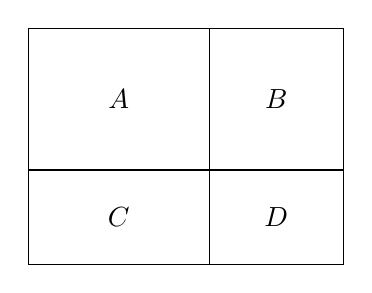
\begin{tikzpicture}[baseline=(current bounding box.center)]
  \draw (0,0) rectangle (4,3);
  \draw (0,1.2) -- (4,1.2);
  \draw (2.3,0) -- (2.3,3);
  \node at (1.15,2.1) {$A$};
  \node at (3.15,2.1) {$B$};
  \node at (1.15,0.6) {$C$};
  \node at (3.15,0.6) {$D$};
\end{tikzpicture}
\]

\begin{proposition}[分块加法与数乘]
大小相容时，分块矩阵的加法与数乘可以逐块进行：
\[
\mat{A&B\\C&D}+\mat{A'&B'\\C'&D'}=
\mat{A+A'&B+B'\\C+C'&D+D'},
\]
\[
\lambda\mat{A&B\\C&D}=
\mat{\lambda A&\lambda B\\\lambda C&\lambda D}.
\]
\end{proposition}

\begin{proof}
这是普通矩阵加法与数乘逐项进行的直接结果。把整个矩阵按照块的边界观察，就得到逐块公式。
\end{proof}

\begin{proposition}[分块乘法]
若块的大小相容，则
\[
\mat{A&B\\C&D}
\mat{E&F\\G&H}
=
\mat{AE+BG&AF+BH\\CE+DG&CF+DH}.
\]
\end{proposition}

\begin{proof}
按普通矩阵乘法定义计算即可。例如左上块由第一行块与第一列块相乘求和得到，即 $AE+BG$。其余三块同理。
\end{proof}

\begin{example}
设
\[
M=\mat{1&2&0\\0&1&3\\0&0&2}
=\mat{egin{matrix}1&2\\0&1\end{matrix}&egin{matrix}0\\3\end{matrix}\\
\begin{matrix}0&0\end{matrix}&(2)}.
\]
把它看成 $2\times 2$ 块矩阵，既可以快速描述其结构，也便于后续使用 Schur 补公式。
\end{example}

\subsection{分块行列式}

\begin{proposition}[分块对角矩阵]
若
\[
M=\mat{A&0\\0&D},
\]
其中 $A\in\Mat_m(\F)$，$D\in\Mat_r(\F)$，则
\[
\det(M)=\det(A)\det(D).
\]
\end{proposition}

\begin{proof}
矩阵 $M$ 是一个普通的块对角矩阵。它实际上也是上三角块矩阵，主对角线上分别是 $A$ 与 $D$。若进一步对 $A$ 与 $D$ 分别做三角化思考，或直接用排列定义，都可看出非零项只能来自“不跨块取元”的排列，因此行列式分解为两部分之积，即
\[
\det(M)=\det(A)\det(D).
\]
更形式化地说，把 $M$ 的前 $m$ 列与后 $r$ 列分开，任何把前 $m$ 行送到后 $r$ 列的排列都会取到零元，所以只剩在各块内部排列的项。
\end{proof}

\begin{proposition}[块上三角矩阵]
若
\[
M=\mat{A&B\\0&D},
\]
其中 $A\in\Mat_m(\F)$，$D\in\Mat_r(\F)$，则
\[
\det(M)=\det(A)\det(D).
\]
\end{proposition}

\begin{proof}
与上一个命题同理。由于左下块为零，Leibniz 公式中任何把后 $r$ 行中的某一行与前 $m$ 列中的某一列配对的排列都会产生零项，因此仅保留分别在 $A$ 与 $D$ 内部排列的项，故结果为两块行列式的乘积。
\end{proof}

\begin{theorem}[Schur 补公式]
设
\[
M=\mat{A&B\\C&D},
\]
其中 $A\in\Mat_m(\F)$ 可逆，则
\[
\det(M)=\det(A)\det(D-CA^{-1}B).
\]
矩阵
\[
D-CA^{-1}B
\]
称为 $A$ 在 $M$ 中的 \emph{Schur 补}。
\end{theorem}

\begin{proof}
考虑分块矩阵
\[
L=\mat{I_m&0\\-CA^{-1}&I_r},
\qquad
R=\mat{I_m&-A^{-1}B\\0&I_r}.
\]
它们都是块下三角或块上三角矩阵，且对角块都是单位矩阵，所以由上一个命题可知
\[
\det(L)=\det(R)=1.
\]
现在直接计算：
\begin{align*}
LMR
&=
\mat{I_m&0\\-CA^{-1}&I_r}
\mat{A&B\\C&D}
\mat{I_m&-A^{-1}B\\0&I_r}\\
&=
\mat{A&B\\0&D-CA^{-1}B}
\mat{I_m&-A^{-1}B\\0&I_r}\\
&=
\mat{A&0\\0&D-CA^{-1}B}.
\end{align*}
于是
\[
\det(M)=\det(LMR)=\det(A)\det(D-CA^{-1}B),
\]
因为乘以 $L,R$ 不改变行列式，而最后一个矩阵是块对角矩阵。
\end{proof}

\begin{remark}
若 $D$ 可逆，也有对称公式
\[
\det(M)=\det(D)\det(A-BD^{-1}C).
\]
在数值线性代数、二次型、表示论乃至模形式的 Hecke 代数研究中，Schur 补都经常出现。本书后续不会频繁使用它，但分块思想会反复出现。
\end{remark}

\begin{example}
设
\[
M=\mat{1&2&1\\0&1&3\\2&0&1}
=
\mat{egin{matrix}1&2\\0&1\end{matrix}&egin{matrix}1\\3\end{matrix}\\
\begin{matrix}2&0\end{matrix}&(1)}.
\]
取
\[
A=\mat{1&2\\0&1},\quad B=\mat{1\\3},\quad C=\mat{2&0},\quad D=(1).
\]
则
\[
A^{-1}=\mat{1&-2\\0&1},
\qquad
CA^{-1}B=\mat{2&0}\mat{1&-2\\0&1}\mat{1\\3}=2.
\]
故 Schur 补为 $1-2=-1$，从而
\[
\det(M)=\det(A)\det(-1)=1\cdot(-1)=-1.
\]
读者可直接按三阶行列式验证这一结果。
\end{example}

\section*{本章小结}

本章建立了今后全书都会使用的几个核心工具：
\begin{itemize}
  \item 矩阵乘法体现复合，转置把“行”与“列”互换；
  \item 初等矩阵把高斯消元改写成乘法操作；
  \item 行列式由排列定义，具有交错多线性与乘法性；
  \item $\det(A)\ne0$ 是方阵可逆的充要条件；
  \item Cramer 法则与伴随矩阵给出逆矩阵和线性方程组解的显式公式；
  \item 分块矩阵揭示了大矩阵中的结构，Schur 补是其代表性工具。
\end{itemize}

从下一章开始，我们将把矩阵背后的“线性空间”与“线性映射”作为抽象对象来研究；但本章的具体计算技巧始终不会离场。

\section*{习题}

以下习题按难度分为三组：基础（\basic）、进阶（\medium）与挑战（\hard）。建议先完整做完基础题，再进入后两组。

\subsection*{基础题（共 30 题）}

\begin{enumerate}[label=\arabic*.]
  \item \basic 设
  \[
  A=\mat{1&-2\\3&0},\qquad B=\mat{4&1\\-1&5}.
  \]
  计算 $A+B,\ 2A-3B$。

  \item \basic 设
  \[
  A=\mat{1&0&2\\-1&3&4},\qquad B=\mat{2&1\\0&-1\\5&2}.
  \]
  计算 $AB$。

  \item \basic 设
  \[
  A=\mat{2&1\\0&3},\qquad B=\mat{1&4\\-2&0}.
  \]
  分别计算 $AB$ 与 $BA$，并验证它们不相等。

  \item \basic 设
  \[
  A=\mat{1&2&3\\0&1&4},\qquad B=\mat{2&0\\1&-1\\3&5},\qquad C=\mat{1\\2}.
  \]
  计算 $(AB)C$ 与 $A(BC)$。

  \item \basic 求所有 $2\times2$ 矩阵 $X$，使得
  \[
  \mat{1&1\\0&1}X=\mat{2&3\\1&4}.
  \]

  \item \basic 设 $A=\mat{a&b\\c&d}$，$x=\mat{x_1\\x_2}$。把 $Ax$ 写成分量形式，并说明它与二元一次线性方程组的关系。

  \item \basic 求下列矩阵的转置：
  \[
  A=\mat{1&2&3\\4&5&6},\qquad B=\mat{0&1\\-1&0\\2&3}.
  \]

  \item \basic 直接验证
  \[
  (A+B)^T=A^T+B^T
  \]
  对下列矩阵成立：
  \[
  A=\mat{1&0\\2&3},\qquad B=\mat{-1&4\\5&2}.
  \]

  \item \basic 设
  \[
  A=\mat{1&2\\3&4\\5&6},\qquad B=\mat{0&1&2\\-1&3&4}.
  \]
  计算 $(AB)^T$ 与 $B^TA^T$。

  \item \basic 判断下列矩阵是否为对称矩阵或斜对称矩阵：
  \[
  \mat{2&1\\1&5},\qquad \mat{0&3\\-3&0},\qquad \mat{1&2\\-2&1}.
  \]

  \item \basic 对矩阵
  \[
  A=\mat{1&2&3\\4&5&6\\7&8&9}
  \]
  依次进行以下初等行变换：交换第 $1,3$ 行；把第 $2$ 行乘以 $-1$；把第 $1$ 行的 $2$ 倍加到第 $2$ 行。写出每一步得到的矩阵。

  \item \basic 写出在 $I_3$ 上执行操作 $R_2\leftrightarrow R_3$ 所得到的初等矩阵，并计算它左乘矩阵
  \[
  A=\mat{1&0\\2&1\\3&4}
  \]
  的结果。

  \item \basic 写出在 $I_3$ 上执行操作 $R_1\leftarrow 5R_1$ 所得到的初等矩阵，并求其逆矩阵。

  \item \basic 写出在 $I_4$ 上执行操作 $R_3\leftarrow R_3-2R_1$ 所得到的初等矩阵，并把它左乘一般矩阵 $(a_{ij})\in\Mat_{4,2}(\F)$，说明发生了什么变化。

  \item \basic 把矩阵
  \[
  A=\mat{1&2\\3&4}
  \]
  通过初等行变换化为单位矩阵，并由此写出 $A^{-1}$。

  \item \basic 计算下列二阶行列式：
  \[
  \dmat{3&1\\2&5},\qquad \dmat{0&-2\\7&4},\qquad \dmat{a&b\\c&d}.
  \]

  \item \basic 计算下列三阶行列式：
  \[
  \dmat{1&2&0\\0&3&4\\5&0&1}.
  \]

  \item \basic 用第一行展开计算
  \[
  \dmat{2&1&3\\0&-1&4\\5&2&0}.
  \]

  \item \basic 用第三列展开计算
  \[
  \dmat{1&0&2\\3&1&4\\-1&2&0}.
  \]

  \item \basic 设
  \[
  A=\mat{1&2\\3&4}.
  \]
  分别计算交换两行、把第一行乘以 $3$、把第二行加上第一行的 $5$ 倍之后所得矩阵的行列式。

  \item \basic 计算下列上三角或下三角矩阵的行列式：
  \[
  \mat{2&1&3\\0&-1&4\\0&0&5},
  \qquad
  \mat{1&0&0\\2&3&0\\4&5&6}.
  \]

  \item \basic 验证
  \[
  \det(A^T)=\det(A)
  \]
  对矩阵
  \[
  A=\mat{1&2&3\\0&1&4\\5&6&0}
  \]
  成立。

  \item \basic 求下列矩阵的逆矩阵：
  \[
  \mat{2&1\\1&1},
  \qquad
  \mat{1&3\\2&5}.
  \]

  \item \basic 利用伴随矩阵公式求
  \[
  A=\mat{1&2\\3&7}
  \]
  的逆矩阵。

  \item \basic 判断下列矩阵是否可逆：
  \[
  \mat{1&2\\2&4},
  \qquad
  \mat{1&0&0\\0&2&0\\0&0&3},
  \qquad
  \mat{1&1&1\\1&1&1\\0&1&2}.
  \]

  \item \basic 用 Cramer 法则求解方程组
  \[
  \begin{cases}
  x+y=3,\\
  2x-y=0.
  \end{cases}
  \]

  \item \basic 用 Cramer 法则求解方程组
  \[
  \begin{cases}
  x+2y+z=1,\\
  2x-y+z=0,\\
  x+y-z=2.
  \end{cases}
  \]

  \item \basic 设
  \[
  M=\mat{A&0\\0&D},
  \qquad
  A=\mat{1&2\\0&1},\quad D=\mat{3&0\\4&5}.
  \]
  计算 $\det(M)$。

  \item \basic 按分块乘法计算
  \[
  \mat{1&0&2\\0&1&3\\0&0&1}
  \mat{1&1&0\\0&1&0\\0&0&2}
  \]
  ，要求先把它们视为 $2\times2$ 块矩阵再计算。

  \item \basic 对矩阵
  \[
  M=\mat{2&1&0\\0&1&3\\4&0&1}
  =\mat{(2)&\begin{matrix}1&0\end{matrix}\\
  \begin{matrix}0\\4\end{matrix}&\begin{matrix}1&3\\0&1\end{matrix}}
  \]
  写出关于左上角块的 Schur 补，并计算其值。
\end{enumerate}

\subsection*{进阶题（共 20 题）}

\begin{enumerate}[label=\arabic*.,start=31]
  \item \medium 设 $A\in\Mat_{m,n}(\F)$，证明 $(A^T)^T=A$ 与 $(\lambda A)^T=\lambda A^T$。

  \item \medium 证明：对任意 $n\ge2$，存在 $A,B\in\Mat_n(\F)$ 使得 $AB\ne BA$。

  \item \medium 设 $A,B\in\Mat_n(\F)$。证明：若 $AB=I_n$，则必有 $BA=I_n$。\emph{提示：可用行列式。}

  \item \medium 证明：每个可逆矩阵都可以写成有限个初等矩阵的乘积。

  \item \medium 设 $A\in\Mat_n(\F)$，证明下列三条初等行变换对行列式的影响分别是：变号、乘以对应倍数、不变。

  \item \medium 只利用“初等矩阵”和“可逆矩阵可分解为初等矩阵乘积”证明
  \[
  \det(AB)=\det(A)\det(B)
  \]
  对所有可逆矩阵成立；再推广到一般矩阵。

  \item \medium 证明伴随矩阵恒等式
  \[
  A\,\operatorname{adj}(A)=\det(A)I_n.
  \]
  并说明为什么也有 $\operatorname{adj}(A)A=\det(A)I_n$。

  \item \medium 讨论参数 $t\in\F$ 取何值时矩阵
  \[
  A_t=\mat{1&t&1\\0&1&t\\t&0&1}
  \]
  可逆，并在可逆时求其行列式。

  \item \medium 证明：任意上三角矩阵的行列式等于其对角元之积。

  \item \medium 设 $A\in\Mat_{m,n}(\F)$，$B\in\Mat_{n,r}(\F)$。证明秩不等式
  \[
  \rank(AB)\le \min\{\rank(A),\rank(B)\}.
  \]

  \item \medium 证明：若 $AB$ 可逆，则 $A$ 与 $B$ 都可逆。

  \item \medium 设 $A,B\in\Mat_n(\F)$，证明函数
  \[
  f(t)=\det(A+tB)
  \]
  是关于 $t$ 的次数不超过 $n$ 的多项式。

  \item \medium 设 $A=(a_{ij})\in\Mat_n(\F)$，证明对任意 $i\ne j$，有
  \[
  \sum_{k=1}^n a_{ik}C_{jk}=0.
  \]

  \item \medium 设分块矩阵
  \[
  M=\mat{A&B\\0&D}
  \]
  ，其中 $A,D$ 为方阵。证明 $M$ 可逆当且仅当 $A,D$ 都可逆，并求 $M^{-1}$ 的分块表达式。

  \item \medium 设
  \[
  A=\mat{1&1\\0&1}.
  \]
  求 $A^n$（$n\in\N$）的显式公式，并由此说明矩阵乘法如何编码递推过程。

  \item \medium 设
  \[
  A=\mat{a&b\\c&d}.
  \]
  证明 $|\det(A)|$ 等于由列向量 $\mat{a\\c}$ 与 $\mat{b\\d}$ 张成的平行四边形面积。

  \item \medium 对任意排列 $\sigma\in S_n$，设 $P_\sigma$ 为对应的置换矩阵。证明
  \[
  \det(P_\sigma)=\sgn(\sigma).
  \]

  \item \medium 设 $A\in\Mat_n(\F)$ 可逆，$b\in\F^n$。证明方程组 $Ax=b$ 的第 $j$ 个分量可以写成
  \[
  x_j=\frac{\sum_{i=1}^n C_{ji}b_i}{\det(A)}.
  \]
  并与 Cramer 法则比较。

  \item \medium 设
  \[
  A=\mat{a&b\\c&d}\in \SL_2(\Z).
  \]
  证明其逆矩阵仍在 $\SL_2(\Z)$ 中，并写出显式公式。

  \item \medium 设 $A\in\Mat_n(\F)$ 满足 $A^T=-A$。证明当 $n$ 为奇数时，$\det(A)=0$。
\end{enumerate}

\subsection*{挑战题（共 10 题）}

\begin{enumerate}[label=\arabic*.,start=51]
  \item \hard 证明 Vandermonde 行列式公式：
  \[
  \det\mat{1&1&\cdots&1\\x_1&x_2&\cdots&x_n\\\vdots&\vdots&\ddots&\vdots\\x_1^{n-1}&x_2^{n-1}&\cdots&x_n^{n-1}}
  =\prod_{1\le i<j\le n}(x_j-x_i).
  \]

  \item \hard 设 $\Phi:(\F^n)^n\to\F$ 是交错多线性函数。证明存在唯一常数 $c\in\F$ 使得
  \[
  \Phi(v_1,\dots,v_n)=c\det(v_1,\dots,v_n)
  \]
  对所有 $v_1,\dots,v_n$ 成立。

  \item \hard 证明 Cauchy--Binet 公式：若 $A\in\Mat_{m,n}(\F)$，$B\in\Mat_{n,m}(\F)$ 且 $m\le n$，则
  \[
  \det(AB)=\sum_{I\subseteq\{1,\dots,n\},\,|I|=m}\det(A_{[:,I]})\det(B_{[I,:]}).
  \]
  这里 $A_{[:,I]}$ 表示由 $A$ 取指标集 $I$ 所对应列得到的 $m\times m$ 子矩阵，$B_{[I,:]}$ 类似。

  \item \hard 利用上一题证明：若 $A\in\Mat_{m,n}(\R)$ 且 $m\le n$，则
  \[
  \det(AA^T)=\sum_{I,\,|I|=m}\det(A_{[:,I]})^2.
  \]

  \item \hard 设
  \[
  S=\mat{0&-1\\1&0},\qquad T=\mat{1&1\\0&1}.
  \]
  对下列列向量分别计算 $S$ 与 $T$ 的作用：
  \[
  \mat{1\\0},\quad \mat{0\\1},\quad \mat{2\\3},\quad \mat{-1\\4}.
  \]
  并解释 $S,T\in\SL_2(\Z)$ 的原因。

  \item \hard 对上题中的矩阵 $S,T$，证明
  \[
  S^2=-I_2,
  \qquad
  (ST)^3=-I_2.
  \]
  从而说明在 $\PSL_2(\Z)=\SL_2(\Z)/\{\pm I_2\}$ 中有关系式 $S^2=(ST)^3=I$。

  \item \hard 设 $\tau$ 属于上半平面
  \[
  \{z\in\C\mid \Im(z)>0\},
  \]
  定义
  \[
  S\cdot\tau=-\frac{1}{\tau},\qquad T\cdot\tau=\tau+1.
  \]
  求出 $S$ 与 $ST$ 在上半平面中的不动点，并解释这些点为何在模形式理论中重要。

  \item \hard 证明：若 $M=\mat{a&b\\c&d}\in\Mat_2(\Z)$ 满足 $\det(M)=1$，则其列向量构成 $\Z^2$ 的一个有向基；反过来，若两个整数列向量构成 $\Z^2$ 的一个有向基，则以它们为列得到的矩阵属于 $\SL_2(\Z)$。

  \item \hard 设
  \[
  M=\mat{A&B\\C&D}
  \]
  为分块矩阵，且 $A$ 可逆。利用初等块变换重新证明 Schur 补公式
  \[
  \det(M)=\det(A)\det(D-CA^{-1}B).
  \]
  并说明它与普通高斯消元的关系。

  \item \hard 设 $A\in\Mat_n(\F)$，证明下列命题等价：
  \begin{enumerate}[label=(\alph*)]
    \item $A$ 可逆；
    \item 存在矩阵 $B$ 使 $AB=I_n$；
    \item 存在矩阵 $C$ 使 $CA=I_n$；
    \item $A$ 可以表示为有限个初等矩阵的乘积；
    \item $\det(A)\ne0$。
  \end{enumerate}
\end{enumerate}
